\section{Introduction}
\label{s:intro}

Inspired by the progress that benchmarking brought to computer vision~\cite{deng2009imagenet,lin2014microsoft,everingham2010pascal,krishna2017visual,geiger2012we,goyal2017something,sigurdsson2018actor,xiang2017posecnn,martin2021jrdb,caba2015activitynet,gurari2018vizwiz} and natural language processing~\cite{marcinkiewicz1994building,wang2018glue,rajpurkar2016squad,socher2013recursive,antol2015vqa}, the robotics community has developed several benchmarks in simulation~\cite{batra2020rearrangement,weihs2021visual,gan2021threedworld,puig2018virtualhome,shridhar2020alfred,xia2020interactive,yu2020meta,james2019rlbench,savva2019habitat,szot2021habitat,srivastava2021behavior,zhu2020robosuite,tassa2018deepmind,brockman2016openai}.
The broader goal of these benchmarks is to fuel the development of general, effective robots that bring major benefits to people's daily lives---human-centered AI that ``serves human needs, goals, and values''~\cite{littman2021gathering, riedl2019human, xu2019toward,shneiderman2020bridging}. Inspiring as they are, the tasks and activities in those benchmarks are designed by researchers; it remains unclear if they are addressing the actual needs of humans. %However, efforts to identify and incorporate activities that are grounded in human needs have been lacking in the field. 

We observe that a human-centered robotic benchmark should not only be designed \emph{for} human needs, but also originated \emph{from} human needs: \textit{what everyday activities do humans want robots to do for them?} % To move toward a human-centered benchmark for embodied AI, we must first address the question: \textit{what everyday activities do humans want robots to do for them?}
%Useful information for guiding the key technical advances can come from surveying human needs directly. 
To this end, we conduct an extensive survey with 1,461 participants (see Sec.~\ref{sec:survey}) to rank a wide range of daily activities based on participants' desire to delegate these activities to robots. We also ask layperson annotators to provide definitions of those activities. The survey reveals systematicity in what activities people want robots to do, but more importantly, highlights two key factors that we should prioritize when designing robotic benchmarks: \textbf{diversity} in the type of scenes, objects, and activities, and \textbf{realism} of the underlying simulation environments. %physical states and processes involved in these activities. By incorporating such knowledge, we develop benchmarks that are diverse, ecological and human-centered, with activities that reflect actual human needs, goals, and values.%, and with the diversity to improve robot learning generalization along the most critical dimensions.

The most needed activities indicated by the survey range from `wash floor' to `clean bathtub.' Clearly, the diversity of these activities is far beyond what real-world robotics challenges may offer~\cite{kitano1997robocup,wisspeintner2009robocup,iocchi2015robocup,buehler2009darpa,krotkov2017darpa,correll2016analysis,eppner2017lessons,roa2021mobile}. %The diversity necessary to cover human needs forces robots to overcome the challenges of generalization. 
Developing simulation environments is a natural alternative: one can train and test robotic agents in many activities with diverse scenes, objects, and conditions efficiently and safely. %, quickly and safely without having to move a real robot.
However, for this paradigm to work, the activities have to be simulated realistically, reproducing accurately the circumstances that a robot may encounter in the real world. %, a common goal of existing embodied AI simulation benchmarks.
While significant progress in realism has been made in specific domains~\cite{heiden2021disect,urakami2019doorgym,lin2020softgym}, achieving realism for a diverse set of activities remains a tremendous challenge, due to the effort required to provide realistic models and simulation features. %Therefore, it is critical to guide this effort by understanding what types of realism are most critical and relevant for developing robots that meet human needs. 


% Achieving realism in simulation for these diverse activities is a significant challenge. 

%such as possible initial conditions, acceptable goal states, sensor observations, actions, and environment's dynamics. 


In this work, we present \textbf{\benchmark}, a Benchmark of 1,000 Everyday Household Activities in Virtual, Interactive, and Ecological Environments---the next generation of \oldbenchmark~\cite{srivastava2021behavior}. 
\benchmark includes two novel components to address the demands for diversity and realism: the diverse \textbf{\dataset} and the realistic \textbf{\simulator} simulation environment. The \dataset is a large-scale dataset comprising 1) a commonsense knowledge base for 1,000 activities with definitions in predicate logic (initial and goal conditions), as well as the objects involved, their properties, and their state transitions, and 2) high-quality 3D assets including 50 scenes and 9,000+ object models with rich physical and semantic annotations. 

All activities in the \dataset are instantiated in a novel simulation environment, \simulator, which we build on top of Nvidia's Omniverse and PhysX 5~\cite{physx} to provide realistic physics simulation and rendering of rigid bodies, deformable bodies, and fluids. 
%We incorporated these most advanced simulation technology into large realistic scenes with diverse task setups. 
%On top of this, 
\simulator expands beyond Omniverse's capabilities with a set of extended object states like temperature, toggled, soaked, and dirtiness. It also includes capabilities to generate valid initial activity configurations and discriminate valid goal solutions based on activity definitions. % in the \dataset with predicates. %such as \texttt{Cooked} or \texttt{Soaked} or \texttt{Cleaned}. 
With all these realistic simulation features, \simulator supports the 1,000 diverse activities in the \dataset.


We evaluate state-of-the-art reinforcement learning algorithms~\cite{schulman2017proximal,haarnoja2018soft} in several activities of \benchmark, both with visuomotor control in the original action space, and with action primitives that leverage sampling-based motion planning~\cite{Jordan.Perez.ea:CSAIL13}. Our analysis indicates that even a single activity in \benchmark is extremely challenging for current AI algorithms, and the baselines can only solve it with a significant injection of domain knowledge. Concretely, the difficulties derive in part from the length of \benchmark's activities and the complexity of the physical manipulation required. To calibrate the simulation-to-real gap of \benchmark, we provide an initial study on transferring solutions learned with a mobile manipulator in a simulated apartment to its real-world counterpart. %We also quantify the simulation-to-real gap in \simulator with extensive experiments on a real-world robotic setup: a mobile manipulator in a realistic apartment that we have accurately modeled in the simulation. We observe that both sensing and actuation noise can cause failures due to their effect on perception, planning, and execution in ways that are not observed in simulation, and provide information to researchers on how to close the gap.
%With its high levels of realism and diversity, w
We hope that the \benchmark benchmark, our survey, and our analysis will serve to support and guide the development of future embodied AI agents and robots.      

\vspace{1cm}

\begin{figure}[t]
    \centering
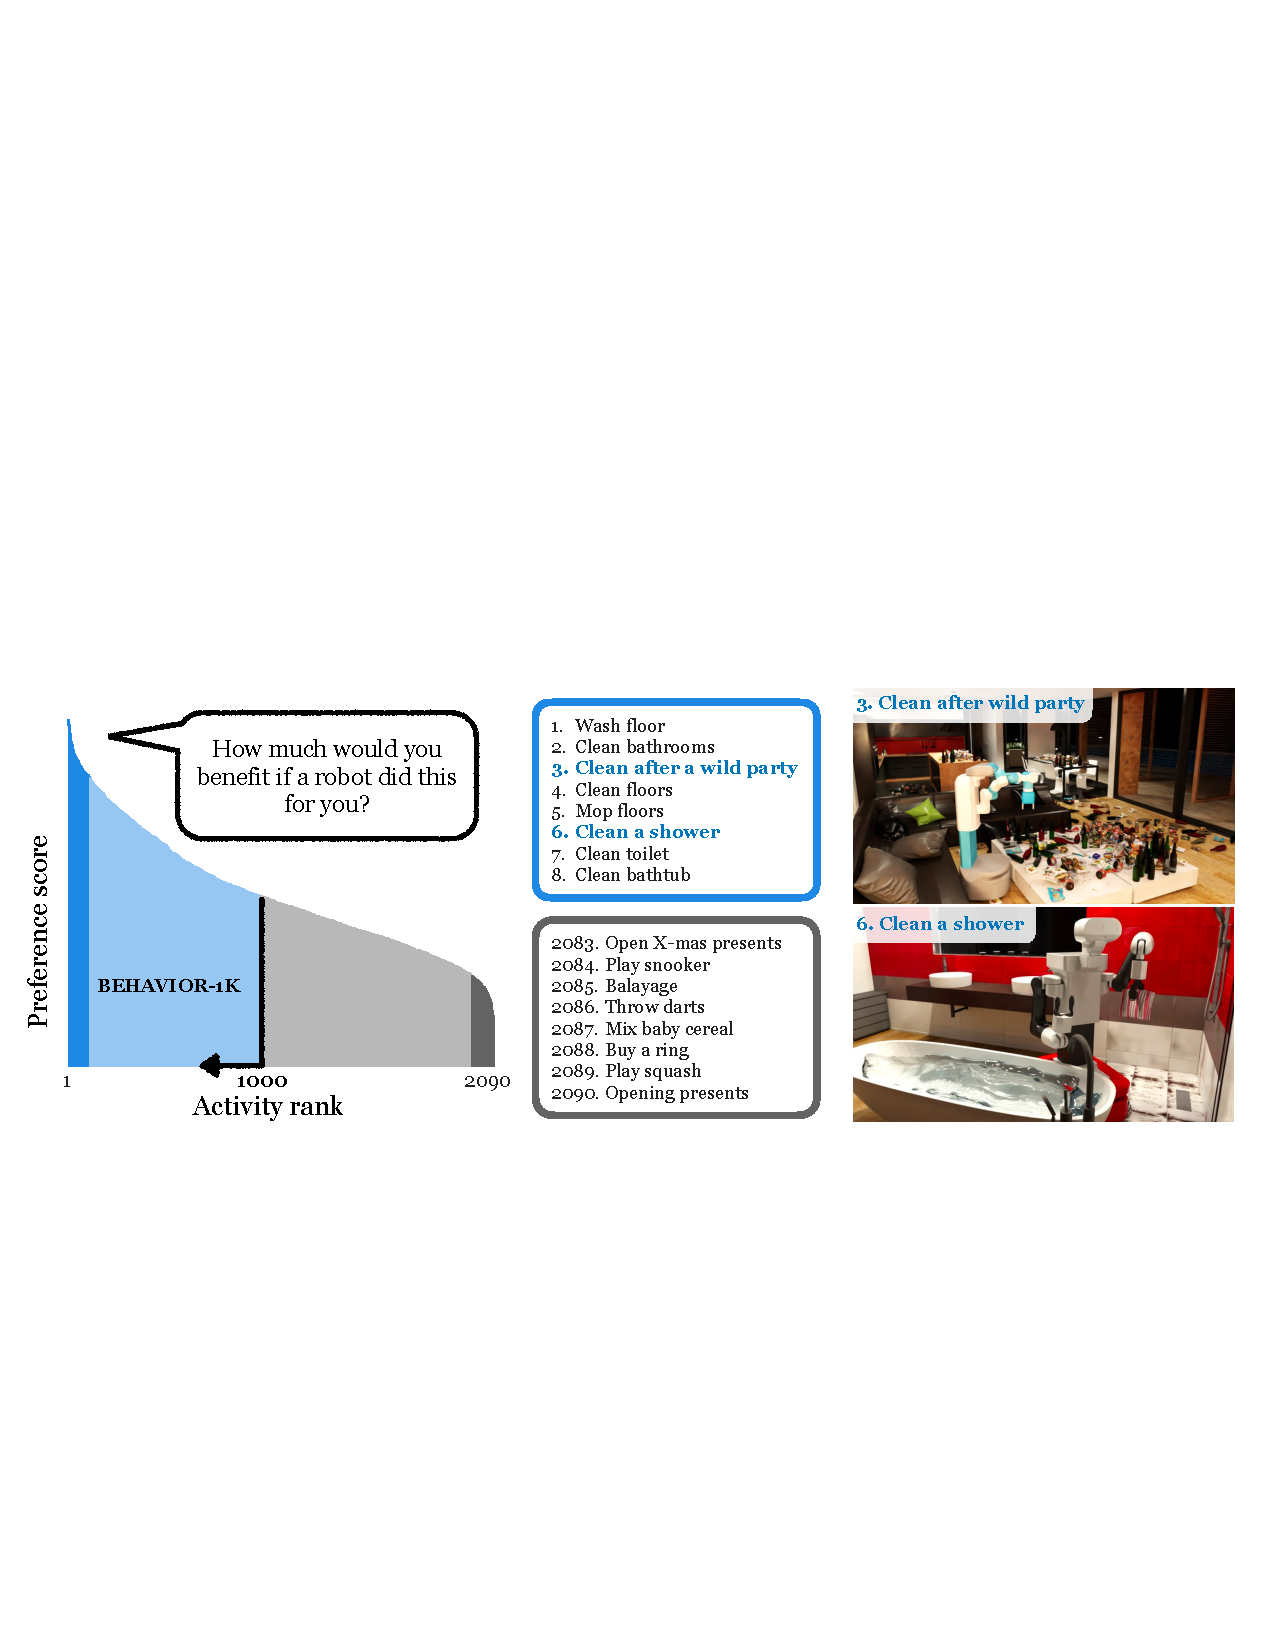
\includegraphics[width=0.99\textwidth]{figures/pull-new.pdf}
\begin{minipage}{0.4\textwidth}
% \includegraphics[width=0.99\textwidth]{figures/survey/all_acts_chart.pdf}
\end{minipage}
%\hfill
% \begin{minipage}{0.58\textwidth}
%  \resizebox{\textwidth}{!}{  
% \begin{tabular}{|c|l|c|l|}
% \hline
% 1 & clean your house after a wild party & 2 & clean a shower \\
% \hline
% 3 & clean grease & 4 & scrubbing bathroom floor \\
% \hline
% 5 & shoveling snow & 6 & washing outside windows \\
% \hline
% 7 & clean walls & 8 & clean up water damage \\
% \hline
% 9 & shovel snow & 10 & clean carpets \\
% \hline
% 11 & clean a grease trap & 12 & emptying trash cans \\
% \hline
% 13 & cleaning pavement & 14 & washing outside walls \\
% \hline
% 15 & washing plates & 16 & sweeping floors \\
% \hline
% 17 & clean the outside of a house & 18 & taking trash outside \\
% \hline
% 19 & clean a couch & 20 & remove hard water spots\\
% \hline
% \end{tabular}
% }
% \end{minipage}
\caption{\textbf{Developing a Human-Centered Benchmark for Embodied AI.} Left: human preference score over 2,090 activities, ranked based on a survey on 1,461 participants. The distribution indicates the high \textbf{diversity} of needs and preferences of humans that should be reflected in a comprehensive benchmark. Middle: Example activities. Laborious activities are ranked the highest, while pleasurable ones are ranked the lowest. Right: visualization of two of the top 8 activities generated by our \textbf{realistic} \simulator simulation environment.}
\label{fig:activity_ranking}
\end{figure}


%%%%%%%% Graveyard of text

%\benchmark is a simulation benchmark for embodied AI and robotics research, which provides realistic simulation of 1000 diverse activities that align with actual human needs. 

% making \simulator one of the most realistic simulators for EAI and robotics research.

% The current AI revolution has been built on top of large benchmarks that provided data and fair conditions to compare solutions~\cite{}. This has been fundamental for the progress in CV~\cite{}, and NLP~\cite{}. However, due to the lack of comprehensive benchmarks, this success has not been yet transferred to some areas of AI. \citet{dehghani2021benchmark} analyzed how the lack of good benchmarking principles for recommendation systems~\cite{} and Atari games~\cite{} is hindering progress and making hard to understand the current state-of-the-art. They call this \emph{rigging the lottery}. In this paper, we present a comprehensive and 



% One of the ultimate goals of these benchmarks is to facilitate the development of smart, effective, robots that facilitate human daily life, i.e., human-centered AIs that ``serve human needs, goals, and values"~\cite{littman2021gathering}. 
% To guide the advances toward this goal, it is critical to have benchmarks that are not only large in scale but that target appropriate tasks, i.e., grounded by actual human needs.
% But, what do humans want robots to do for them? What tasks should we benchmark on?
%\ruohan{realism}To effectively benchmark embodied AI agents in simulation, these benchmarks strive to provide \emph{realistic} simulation that poses similar challenges to those in the real world. %Benchmarks that are not rigorously grounded in actual human needs may pose the risk of driving the community further away from the aforementioned goal.
% What do we benchmark
% Developing a realistic simulator require significant effort, hence we may ask: what tasks should be simulated?


%In our path towards a human-centered benchmark for embodied AI, we need to gain knowledge about the question: \textit{what everyday activities do humans want robots do for them?} We conducted a first-of-its-kind survey with 1,412 participants (details in Sec.~\ref{sec:survey}). The results indicate a clear preference to delegate laborious tasks to robots. However, we also observed that the preferences from humans are extremely \textbf{diverse}, covering a wide range of daily activities. Moreover, we further asked humans to provide definitions of those activities, and this revealed further diversity in type of scenes, objects, physical states, and physical transitions involved. Such diversity is not covered by the existing embodied AI benchmarks. A new, human-centered benchmark needs thus to include a wide range of activities in ecologically diverse settings, pushing robots to overcome the key challenge of learning to generalize.

%Generalization can be more easily developed and tested in simulation. However, towards this goal, an important aspect for a simulation benchmark to enable progress in robotics is to be \textbf{realistic}: it needs to accurately reproduce the characteristics of problems that a robot could encounter in the real-world. While significant advances have been done in benchmarks for specific tasks~\cite{heiden2021disect,urakami2019doorgym,lin2020softgym}, achieving realism for a diverse set of activities is a tremendous challenge due to scientific and engineering effort to provide models, simulation and features. Hence guiding such effort towards realistically simulating a diverse set of activities that are grounded by human needs is important.  

% Generalization is a key goal of AI research, and it is easier to develop and test more general agents in simulation.

% These benchmarks aim to help the development of smart, effective robots that facilitate human daily life -- human-centered AIs that ``serve human needs, goals, and values''~\cite{littman2021gathering, riedl2019human, xu2019toward,shneiderman2020bridging}. Advancing toward this goal requires benchmarks with appropriate tasks, grounded in actual human needs, but this information has been so far missing. %leaving the selection of activities to the criteria of the developers.